\documentclass[12pt]{article}

\usepackage{amsmath}
\usepackage{amssymb}
\usepackage{calc}
\usepackage{units}
\usepackage{graphicx}
\usepackage[pdftex]{hyperref}
\usepackage{subfig}
\usepackage[margin=1in]{geometry}
\usepackage{listings}
\usepackage[numbers,sort&compress]{natbib}
\usepackage{bm}
\usepackage{paralist}
\usepackage[draft]{fixme}
\usepackage{textcomp}
\usepackage{yorkdefs}

\newcommand{\halflife}{\ensuremath{T_{\nicefrac{1}{2}}}\xspace}

\hypersetup{
  breaklinks=true,
  pdftitle={Alternating Current RL Circuits},
  pdfauthor={Kevin R. Lynch based on a lab by D.C.Jain}, 
  pdfsubject={Phyiscs, Electricity and magnetism},
  pdfkeywords={resistance, inductance, alternating current},
  pdflang={en-US},
}

\title{Alternating Current RL Circuits}
\author{}
%Kevin R. Lynch, based on an earlier lab by D.C.Jain
%\date{2012-03-12}
\date{}

\begin{document}

\maketitle

\section{Objectives}
\label{sec:objectives}

\begin{enumerate}
\item To understand the voltage/current phase behavior of RL circuits
  under applied alternating current voltages, and
\item To understand the current amplitude behavior of RL circuits
  under applied alternating current voltages.
\end{enumerate}

\section{Introduction}
\label{sec:introduction}

You have studied the behavior of RC circuits under both direct
and alternating current conditions.  The final passive

\begin{figure}
  \centering
%  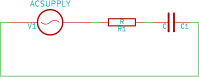
\includegraphics[width=2\textwidth/3]{figures/rc-circuit}
  \caption{The RL circuit.}
  \label{fig:rlcircuit}
\end{figure}
In a previous lab\footnote{\textit{Alternating Current RC Circuits}}
you studied the behavior of the RC circuit under alternating applied
(or AC) voltages.  Here, you will study the behavior of a similar
circuit where the capacitor is replaced with an \textit{inductor}; see
Figure~\ref{fig:rlcircuit}. 

\section{Theory}
\label{sec:theory}

\section{Procedures}
\label{sec:procedures}


\appendix

\section{Derivation of Solutions}
\label{sec:solutions}


\newpage

\section*{Pre-Lab Exercises}

Answer these questions as instructed on Blackboard; make sure to
submit them before your lab session!

\begin{enumerate}
\item Foobar
\end{enumerate}

\newpage

\section*{Post-Lab Exercises}

\begin{enumerate}
\item Discuss briefly whether you have met the objectives of the lab
  exercises.
\end{enumerate}

\end{document}

%%% Local Variables: 
%%% mode: latex
%%% TeX-master: t
%%% End: 
